\subsection{Sequence Diagram}

\begin{figure}[h]
    \centering
    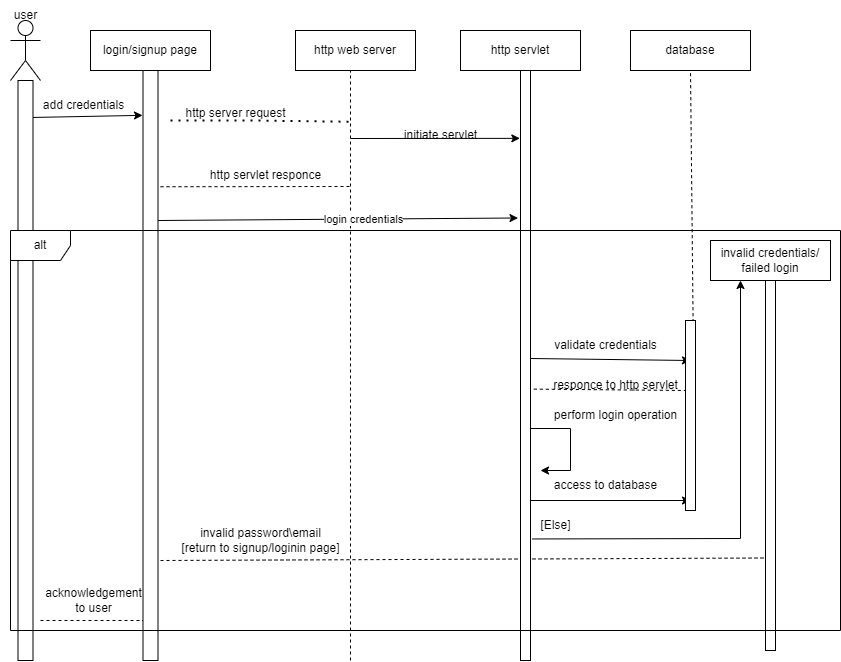
\includegraphics[width=1\textwidth]{images/SD.png}
    \caption{Sequence Diagram}
    \label{FBPM}
\end{figure}

Here it is the sequence diagram for login operation. according to this diagram, user first add his login credentials on the login page and click login. then http web server will initiate the web servlet and carry login credentials towards web servlet. web servelet will responce login page eirther the login is successful or not. web servlet will validate the credentials with database and perform a simple login operation. if the credentials match with the information in the database the login operation will execute and user can access database and have access to dashboard.in other case, if the credentials will not match with database web servlet will redirect the user to login page by and display error message " invalid email or password". and user can acknowledge the problem by error message.